\documentclass{article}
\usepackage{graphicx} % for images

\title{Vehicle Insurance Fraud Modeling Executive Summary}
\author{Sean Murphy}
\date{August 2024}

\begin{document}

\maketitle

\section{Introduction}

Insurance companies strive to provide their clients with reliable coverage in the case of a vehicle 
accident.  Insurance claim fraud, however, undermines their ability to do that.  Although a small 
proportion of claims are fraudulent, an insurance company must recognize when they are.  Otherwise, 
they can cost insurance companies exorbitant amounts of money each year.  Because fraudulent claims 
comprise a small proportion of all claims, developing a statistical model to accurately predict 
fraud is challenging.  This analysis aimed to meet that challenge.   

The data set contained $15,420$ vehicle insurance claims, whether they were fraudulent, and 32 
predictors describing date information, accident information, insurance policy details, and some 
demographics of the people involved.  Although the data were from $1994-96$, a successful analysis 
could provide a case study for insurance companies to use as they address the imbalanced data 
prevalent in the industry.  The four models employed to predict fraud were logistic regression, 
XGBoost, radial kernel SVM, and single-layer artificial neural networks, with various values of 
their respective tuning parameters. 

\section{Data Cleaning}

% introduce age histogram
\begin{figure}
    \centering
    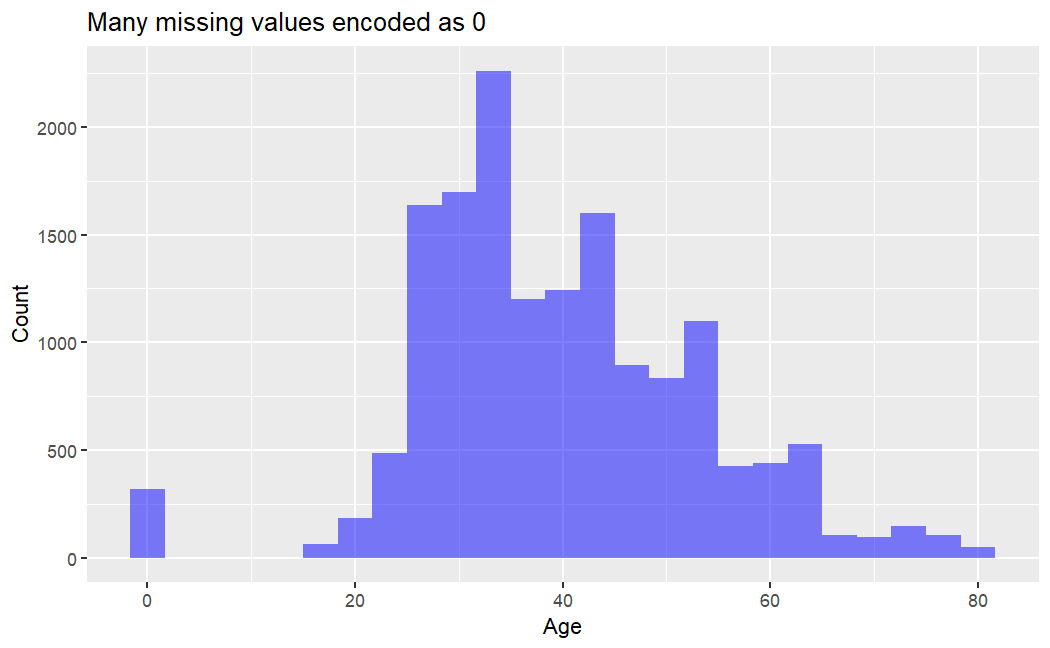
\includegraphics[scale = 0.7]{age_distribution.png}
    \caption{Many missing age values encoded as 0.}
    \label{fig:age_dist}
\end{figure}

The data cleaning proved surprisingly extensive for this project.  While no missing data was encoded 
as $NA$, missing data values were encoded as 0.  For instance, in Figure~\ref{fig:age_dist}, many 
ages are encoded as $0$, indicating missing age column values.  Since these rows with missing age 
values only comprised about $2\%$ of the data and couldn't be reasonably estimated, I removed them 
from the data set.  After removing these values, I log-transformed the age column to reduce skew.  

% introduce conditional prob plot
\begin{figure}
    \centering
    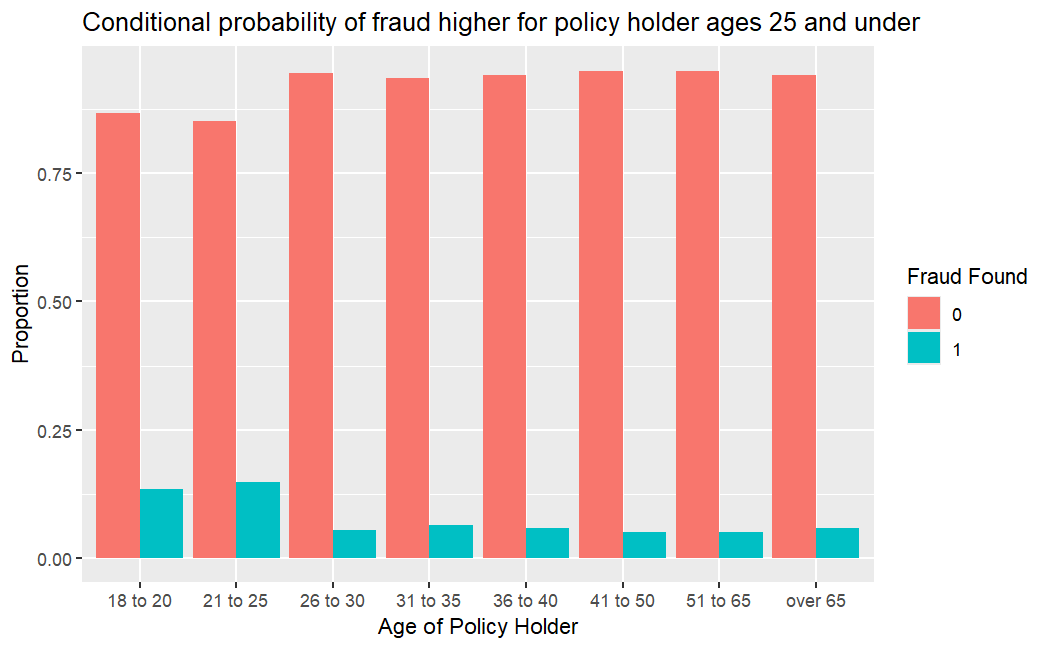
\includegraphics[scale = 0.7]{conditional_prob_age_policyholder.png}
    \caption{Conditional probability pattern indicates age of policy holder should be split into a 
    binary feature depending on whether the age is above or below 25.}
    \label{fig:age_policyholder}
\end{figure}

After initial attempts to train the models had excessively high run times, I sought to reduce the 
dimensionality of the data.  In particular, because most predictors were categorical, I had to 
eliminate unimportant predictors or reduce categories to binaries.  I did this by examining the 
conditional probability of fraud given each category within a categorical predictor and looking 
for patterns.  When the conditional probability of fraud was consistent across categories, that 
feature was dropped.  When the conditional probability of fraud was inconsistent across categories, 
the feature was either kept as-is or reduced to fewer categories.   Figure~\ref{fig:age_policyholder} 
displays a good example of reducing a multi-category feature to a binary when examining the 
conditional probability of fraud based on the policy holder's age. After reducing dimensions, the 
data set contained 18 predictors with no more than 4 categories in any predictor.  I scaled the log 
of age feature since it was the only numeric predictor and then proceeded to identify the proper 
tuning parameter ranges.

\section{Tuning Parameters}

There were many tuning parameters to consider for these four models.  Due to training time limitations, 
only a small range of tuning parameter values could be selected for each model.  I did not consider 
any tuning parameters for logistic regression.  For the XGBoost model, I set the number of trees to 
$100$, the learning rate to a moderate $0.3$, did not include pruning, and tested tree depths of $1$, 
$5$, $10$, $20$, $30$, and $40$.  I kept the minimum child weight small at $1$, used a low sample of 
predictors for each tree at $0.5$ due to the high dimensionality, and started with using all the rows 
at each tree because there were a modest number of observations in the cleaned data set (just over 
$15,000$).  

For the radial SVM, I chose a parameter grid that included cost values $0.01$, $1$, and $100$ to test 
a wide range with a few values tested.  I also included $\sigma$ values of $0.5$ and $3$ to examine 
the optimal degree of fit for the decision boundary.

For the neural network, I included only one layer with $1$, $5$, or $20$ nodes to test the performance 
of models with different layer complexity.  Since the input layer had a size of $27$ and the output 
layer had a size of $1$, I chose node values within this range.  For the decay parameter $\lambda$, 
I chose values of $10$ raised to evenly-spaced powers, $-3$, $-1$ and $1$, to determine the optimal 
weight regularization.

\section{Best Model and Interpretation}

To select the best model, I used 5-fold cross-validation to fit each model using their respective 
tuning parameter grids.  Before cross-validation, I reserved $20\%$ of the data as a holdout set for 
an outer layer of validation, which I will discuss later.  Since the data set was imbalanced, I used 
Cohen's Kappa as the selection metric instead of accuracy.  Accuracy values are poor selection metrics 
for imbalanced data because even a model that uses no predictors can achieve high accuracy by 
predicting that every observation belongs to the majority class. However, this simple model would fail 
to detect every instance of fraud, making it useless.  What is more important is to find a model that 
improves upon a model utilizing no information.  Cohen's Kappa does this well by measuring the 
improvement a model makes over a model that randomly predicts observations according to outcome class 
proportions.   

Using Cohen's Kappa as the metric, I found that an XGBoost model with a tree depth of 30 was optimal, 
with a cross-validated Cohen's Kappa value of $0.126$.  I then fit this model to the entire data set.   

% introduce variable importance plot
\begin{figure}
    \centering
    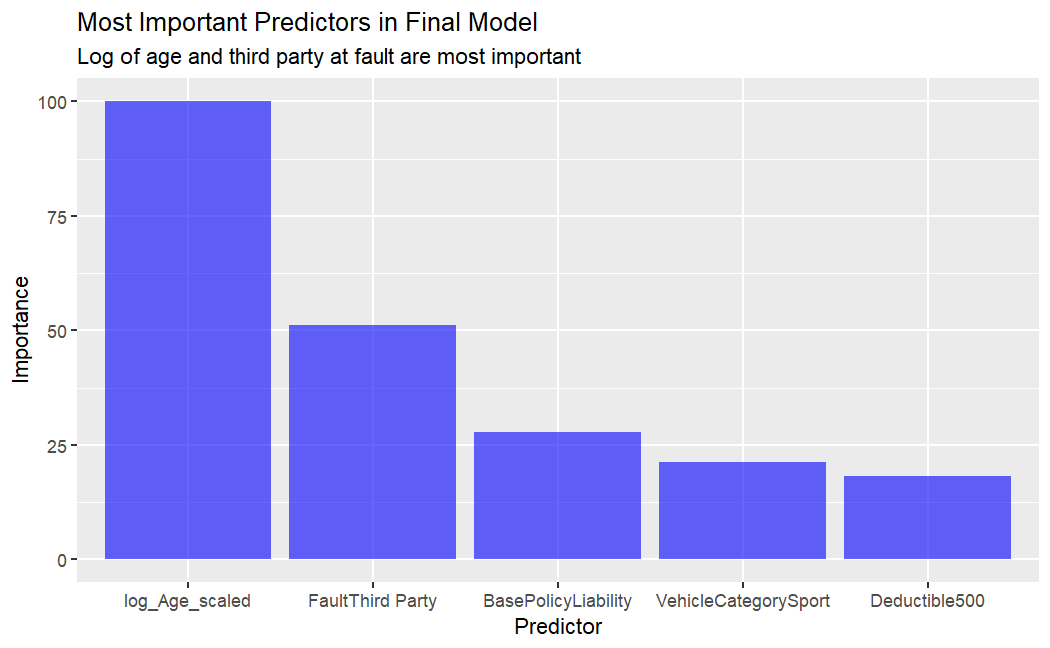
\includegraphics[scale = 0.7]{variable_importance.png}
    \caption{Top 5 most important variables in the final XGBoost model.}
    \label{fig:var_imp}
\end{figure}

After fitting the final model to the entire data set, I examined the variable importance measures.  
The two most important variables in the model were the log of age and the indicator for whether the 
party at fault was a third party, as seen in Figure~\ref{fig:var_imp}.   

% introduce important variables plot against fraud probability
\begin{figure}
    \centering
    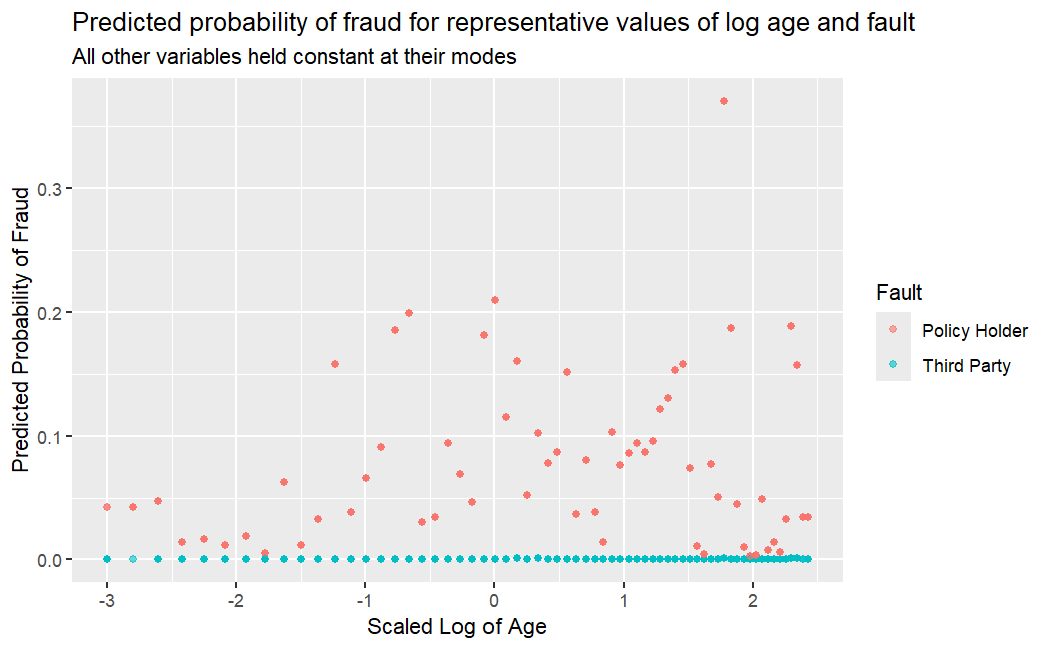
\includegraphics[scale = 0.7]{predicted_probs_important_vars.png}
    \caption{Predicted fraud probability against important predictors holding other predictors 
    constant at their modes.}
    \label{fig:pred_probs}
\end{figure}

To examine the relationship of these variables with the predicted probability of fraud in the final 
XGBoost model, I produced the scatter plot in Figure~\ref{fig:pred_probs}.  This plot indicates that 
there is likely some interaction between age and the party at fault.  When the party at fault is a 
third party, the XGBoost model predicts that the claim is not fraudulent. However, when the party at 
fault is the policyholder, the predicted probability of fraud increases.  Interestingly, as age 
increases, the model also predicts a slight increase in the likelihood of fraud as long as the 
policyholder is at fault. When a third party is at fault, the age does not affect the predicted 
probability of fraud.

Intuitively, it makes sense that the policyholder being at fault increases the probability of fraud.  
It is much more difficult to falsify an insurance claim if you will be pinning the fault on a third 
party.  This typically requires a driving maneuver that intentionally causes an accident while making 
it seem like the other person caused it.  On the other hand, it is much easier for a person to damage 
their own vehicle or report it stolen to get a payout.   

The model's use of age as a predictor is somewhat surprising. I would have intuited that younger 
policyholders would be more likely to commit insurance fraud than older policyholders.  However, the 
model predicts the opposite as long as the policyholder is at fault.  Initially, I would have suspected 
that predictors like police reports and witnesses would have played a far more prominent role in 
determining the probability of fraud than age.  It may be that age plays such a significant role in the 
model because it is the sole numeric predictor and has the most variability in terms of possible values.

\section{Accuracy of Model Fitting Process}

% introduce ROC curves
\begin{figure}
    \centering
    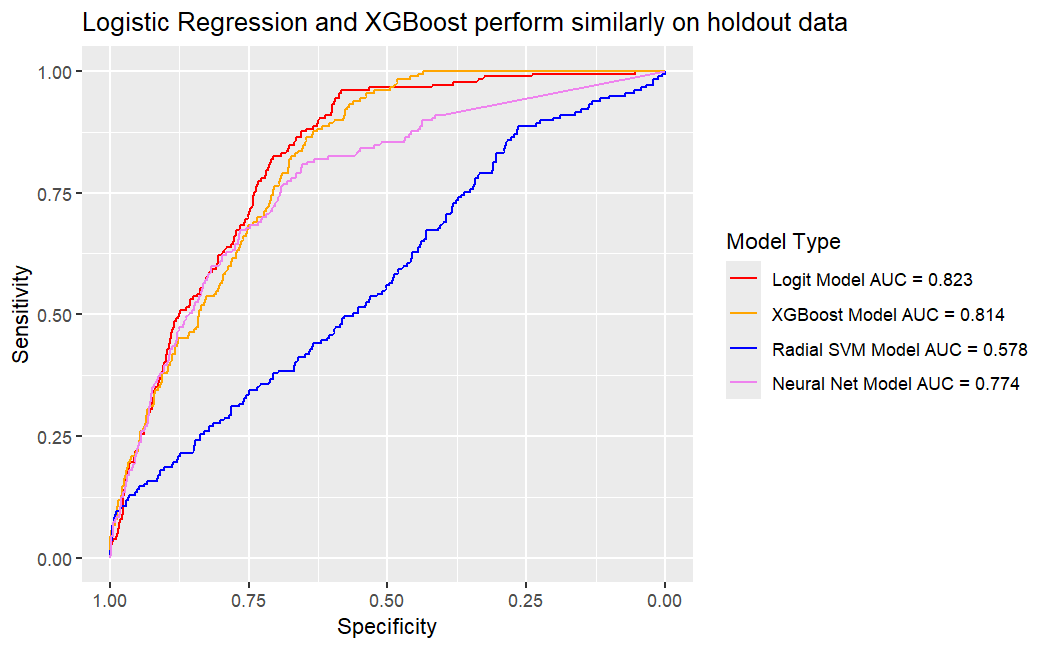
\includegraphics[scale = 0.7]{roc_curves.png}
    \caption{ROC curves of the four models used to predict the holdout set.}
    \label{fig:roc}
\end{figure}

The final stage in this process was assessing the accuracy of the model fitting process.  Due to the 
time it took to train the machine learning models, I used the holdout set approach instead of outer 
cross-validation.  Thus, for each of the models that I fit initially using 5-fold cross-validation, 
I tested the model's performance on the holdout set.  Since accuracy is not a good metric for overall 
performance on this data set, I computed Cohen's Kappa values for each model and plotted their ROC 
curves in Figure~\ref{fig:roc}.  Interestingly, the highest Cohen's Kappa value was for the neural 
network model at $0.101$, and the highest area under the ROC curve was $0.823$ for the logistic 
regression model.  These are the best estimations for the performance of the best model on truly new 
data.

Unfortunately, the best model here is likely not sufficiently accurate to predict vehicle insurance 
fraud reliably.  The best holdout validation Cohen's Kappa value of $0.101$ is only a slight improvement 
on random guessing according to outcome class proportions.  Perhaps more importantly, the best F1 score 
on the holdout set was $0.127$ (neural network model), the harmonic mean between precision and recall.  
Precision measures the proportion of a model's fraud predictions that were correct, while recall measures 
the proportion of fraudulent claims detected by the model.  Since an insurance company would be interested 
in maximizing these quantities, a low F1 score of $0.127$ is not a sufficient indication of a reliable 
model.   

While the current model may not be perfect, there is significant potential for improvement in the future. 
Implementing an upsampling or stratified sampling method could be a promising avenue to explore. This 
could ensure there are enough fraud observations in each cross-validation fold when training the models. 
While it may not have been necessary for this analysis, given the expected $143$ fraud observations in 
each fold, it could certainly be worth trying in the future, especially on more heavily imbalanced data. 
Another strategy to improve performance would be to test a wider range of tuning parameter values.  The 
radial SVM model was not well-suited to this classification task.  Since it took such a long time to 
train, it could be excluded.  This would free up training time to test a wider search grid of tuning 
parameter values for the other models.  In particular, it may also be useful to train neural network 
models containing more than one hidden layer, as a more complex model may pick up on interactions latent 
in the feature space. 
  
This analysis has not yielded a sufficiently accurate model to detect vehicle insurance fraud. However, 
it has shed light on some of the difficulties of this task and on some of the important predictors to 
include in such a task.  It has also revealed some ways the modeling process may be improved to produce 
a satisfactory model.  Predicting insurance fraud is a notably difficult task, but one a robust machine 
learning approach may yet be able to handle.     

\end{document}